\chapter{多维源代码表征学习方法总体设计}
\label{chap:design}

本章首先阐述了当前代码表征学习面临的一些关键技术挑战,进而针对现有的问题提出面向代码克隆检测的多维源代码表征方法RLCCD。然后就该框架的总体架构和处理流程进行详细阐述,最后,给出了下游代码克隆检测任务的问题定义,针对RLCCD框架给出了形式化描述。

\section{代码表征学习面临的技术挑战}
\label{sec:challenges}
目前已有的代码克隆检测方法大多遵循以下思路:(1)首先对代码片段进行预处理;(2)对处理好的代码片段进行代码表征,将其转换为中间表征;(3)根据表征的方式不同计算不同代码片段之间的相似度,完成克隆检测任务。在代码克隆检测中,源代码表征方式决定了信息抽取的程度和粒度,进而影响了后续克隆检测的精度和效率。如何得到丰富且有效的源代码表征表示,是解决代码克隆检测任务的关键所在。从目前多种维度的代码表征方法来看,现有的代码表征方式存在以下技术挑战:

(1)Token维度代码表征存在集外词问题

基于Token的方法一般会利用词法分析器将源代码中的词汇单元Token划分出来,得到Token序列,并过滤掉无用的空格、注释、字符等,然后利用深度学习技术对其进行建模,生成具有丰富代码信息的表征向量,应用于下游代码任务。这类方法和自然语言处理(NLP)领域中常用来处理文本的方式很相似,产生一个规模巨大且稀疏的词汇表。但是,在大多数基于Token的代码克隆检测工具中,通常会将词法单元规范化,例如:将变量名用统一的标识符来代替。经过规范化Token产生的词汇表较小,导致模型学习能力有限,并且在训练过程中会出现未见过或未包含在词汇表中的词语。这些词语可能是用户自定义词、拼写错误、缩写、专有名词等。由于模型在训练阶段没有足够的信息来学习这些词语的表示,因此在实际应用中无法正确处理这些词语,从而导致模型的性能下降,这就是集外词(Out of vocabulary,简称OOV)问题。集外词问题会对模型的性能和泛化能力造成影响,严重限制了代码表征的有限性。

(2)树维度代码表征存在梯度消失问题

基于树的方法将代码通过语法解析转换成相应的抽象语法树,从而有效地表示代码的语法及其结构信息。与自然语言处理领域的长文本类似,当上下文序列很长的时候,基于树的神经网络模型容易出现梯度消失的问题,即梯度在训练过程中变得越来越小,特别是当树非常深的时候,模型会面临梯度消失问题。目前大多数基于树的代码克隆检测方法为了简化或者提高效率,通常会将生成的抽象语法树转换为完整的二叉树,在转换的过程中,不仅破坏了源代码原有的语法结构,也会增加树的高度,进一步削弱模型捕捉复杂语义的能力,导致检测性能下降。

(3)图维度代码表征存在规模开销问题

基于图的方法会将源代码表征为数据流图或者控制流图,数据流图代表了源代码中数据的走向,控制流图代表了代码中语句执行时的跳转流向。大多数基于图的代码克隆检测工具任务的核心是将图中的每个节点映射到一个低维、稠密的特征向量中,并将这些特征编码为特征矩阵,这一步通常需要大量空间开销。同时子图匹配算法是NP完全问题,计算成本过长,时间复杂度很高,因此图维度代码表征学习会存在算法计算开销大,可扩展性不好,检测结果召回率低等问题。

(4)代码表征存在信息利用不充分问题

虽然目前代码表征在Token、树、图等多种维度的研究已经取得了一定的进展,但还存在信息利用不充分的问题。代码不仅仅具有文本自然性,同时具有结构信息、语义信息。在现有的表征粒度中,Token维度的代码表征通常只关注文本自然性,抽象语法树可以捕获程序的语法结构和模式,程序依赖图可以表达程序的部分语义信息,只使用单个特征来表示代码是远远不够的,很难覆盖所有信息,因此存在信息利用不充分,特征表达不完善的问题。

\section{RLCCD研究方案}
\label{sec:Framework}

\subsection{研究思路及总体框架}
\label{subsec:Ideas}
针对\ref{sec:challenges}节提出的四个技术挑战,本文提出了如图\ref{fig:thinking}所示的研究思路。

具体地,本文主要针对代码表征学习的三个维度展开研究工作:(1) 针对Token序列特征挖掘,提出预训练增强辅助模型提取属性特征,从而解决传统基于Token序列的方法存在的集外词问题;(2)针对抽象语法树AST特征挖掘,提出子树划分的改进方法提取结构特征,从而解决传统基于抽象语法树的方法存在的梯度消失问题;(3)针对程序依赖图PDG特征挖掘,提出过滤机制提取语义特征,通过收集PDG的简单特征来过滤输入神经网络模型的输入,从而解决传统基于程序依赖图的方法存在的规模开销问题。

同时,考虑到经由不同表征方式处理所得到的信息通常具有互补性,且不同维度的特征都是代码表示的平行语料,具有信息等价性,因此,本文提出基于多模态学习的特征融合方法,通过融合多个代码特征,包括非结构化(顺序Token形式的代码)和结构化(抽象语法树和程序依赖图形式的代码)信息,从多维数据中学到更好的特征表示,从而有利于提高下游代码克隆检测任务的检测精度。

\begin{figure}[H]
    \centering
    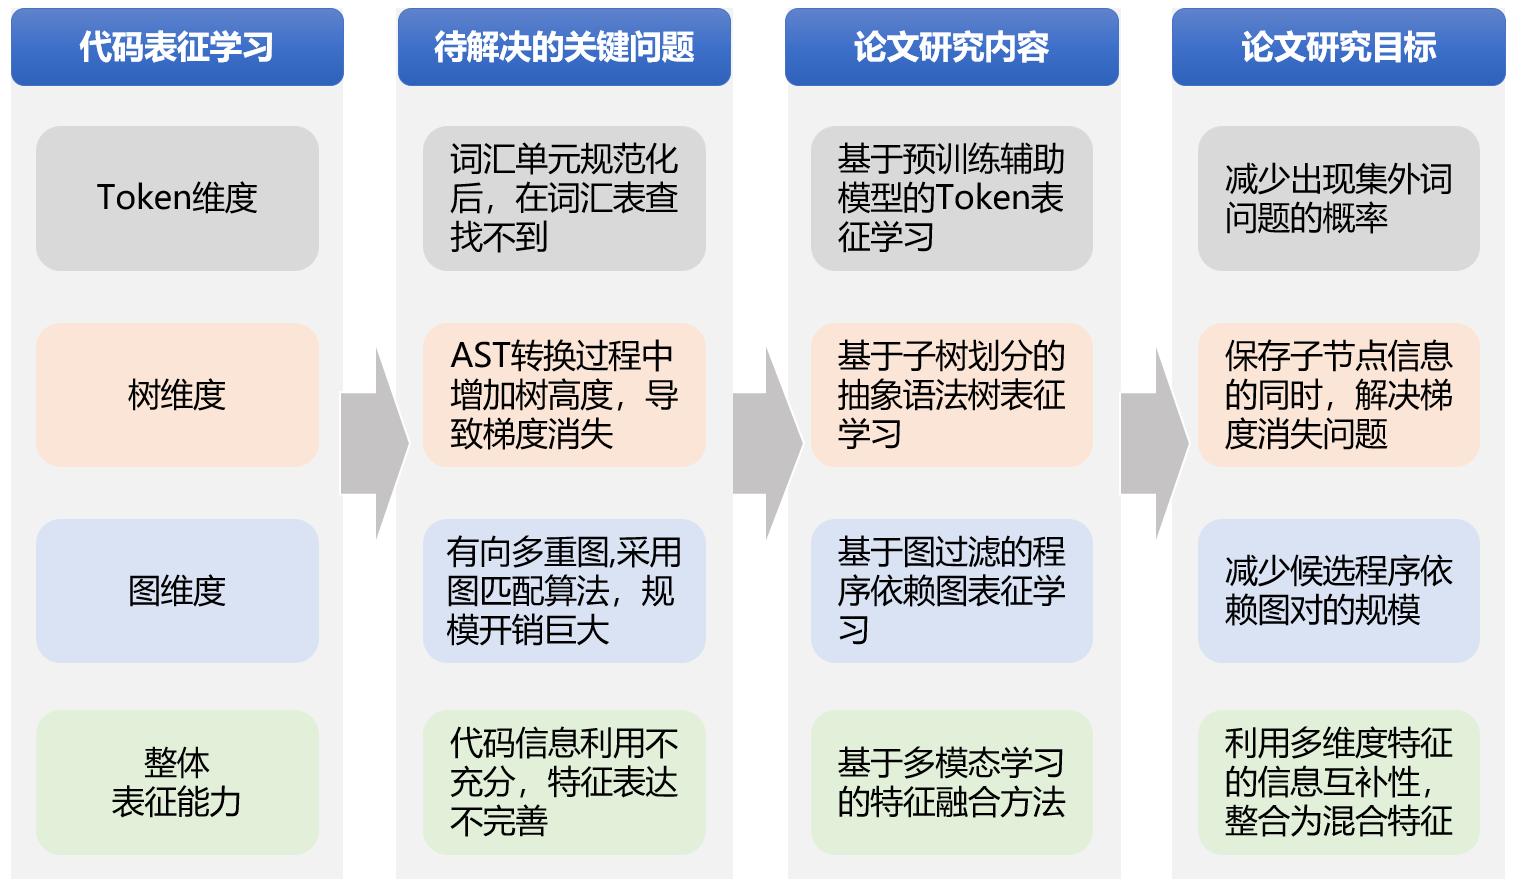
\includegraphics[width=0.75\textwidth]{figures/thinking}
    \caption{研究思路}
    \label{fig:thinking}
\end{figure}

本文基于上述研究思路,设计了面向代码克隆检测的多维源代码表征方法RLCCD,框架如图\ref{fig:framework}所示。由图\ref{fig:framework}可见,本文提出的基本框架与\ref{subsec:Code clone detection}节提出的代码克隆检测的处理流程基本一致,并主要通过三个维度对代码表征学习环节进行改进,然后对三个维度得到的特征向量进行特征融合,得到的混合特征应用到下游代码克隆检测任务中。

\begin{figure}[H]
    \centering
    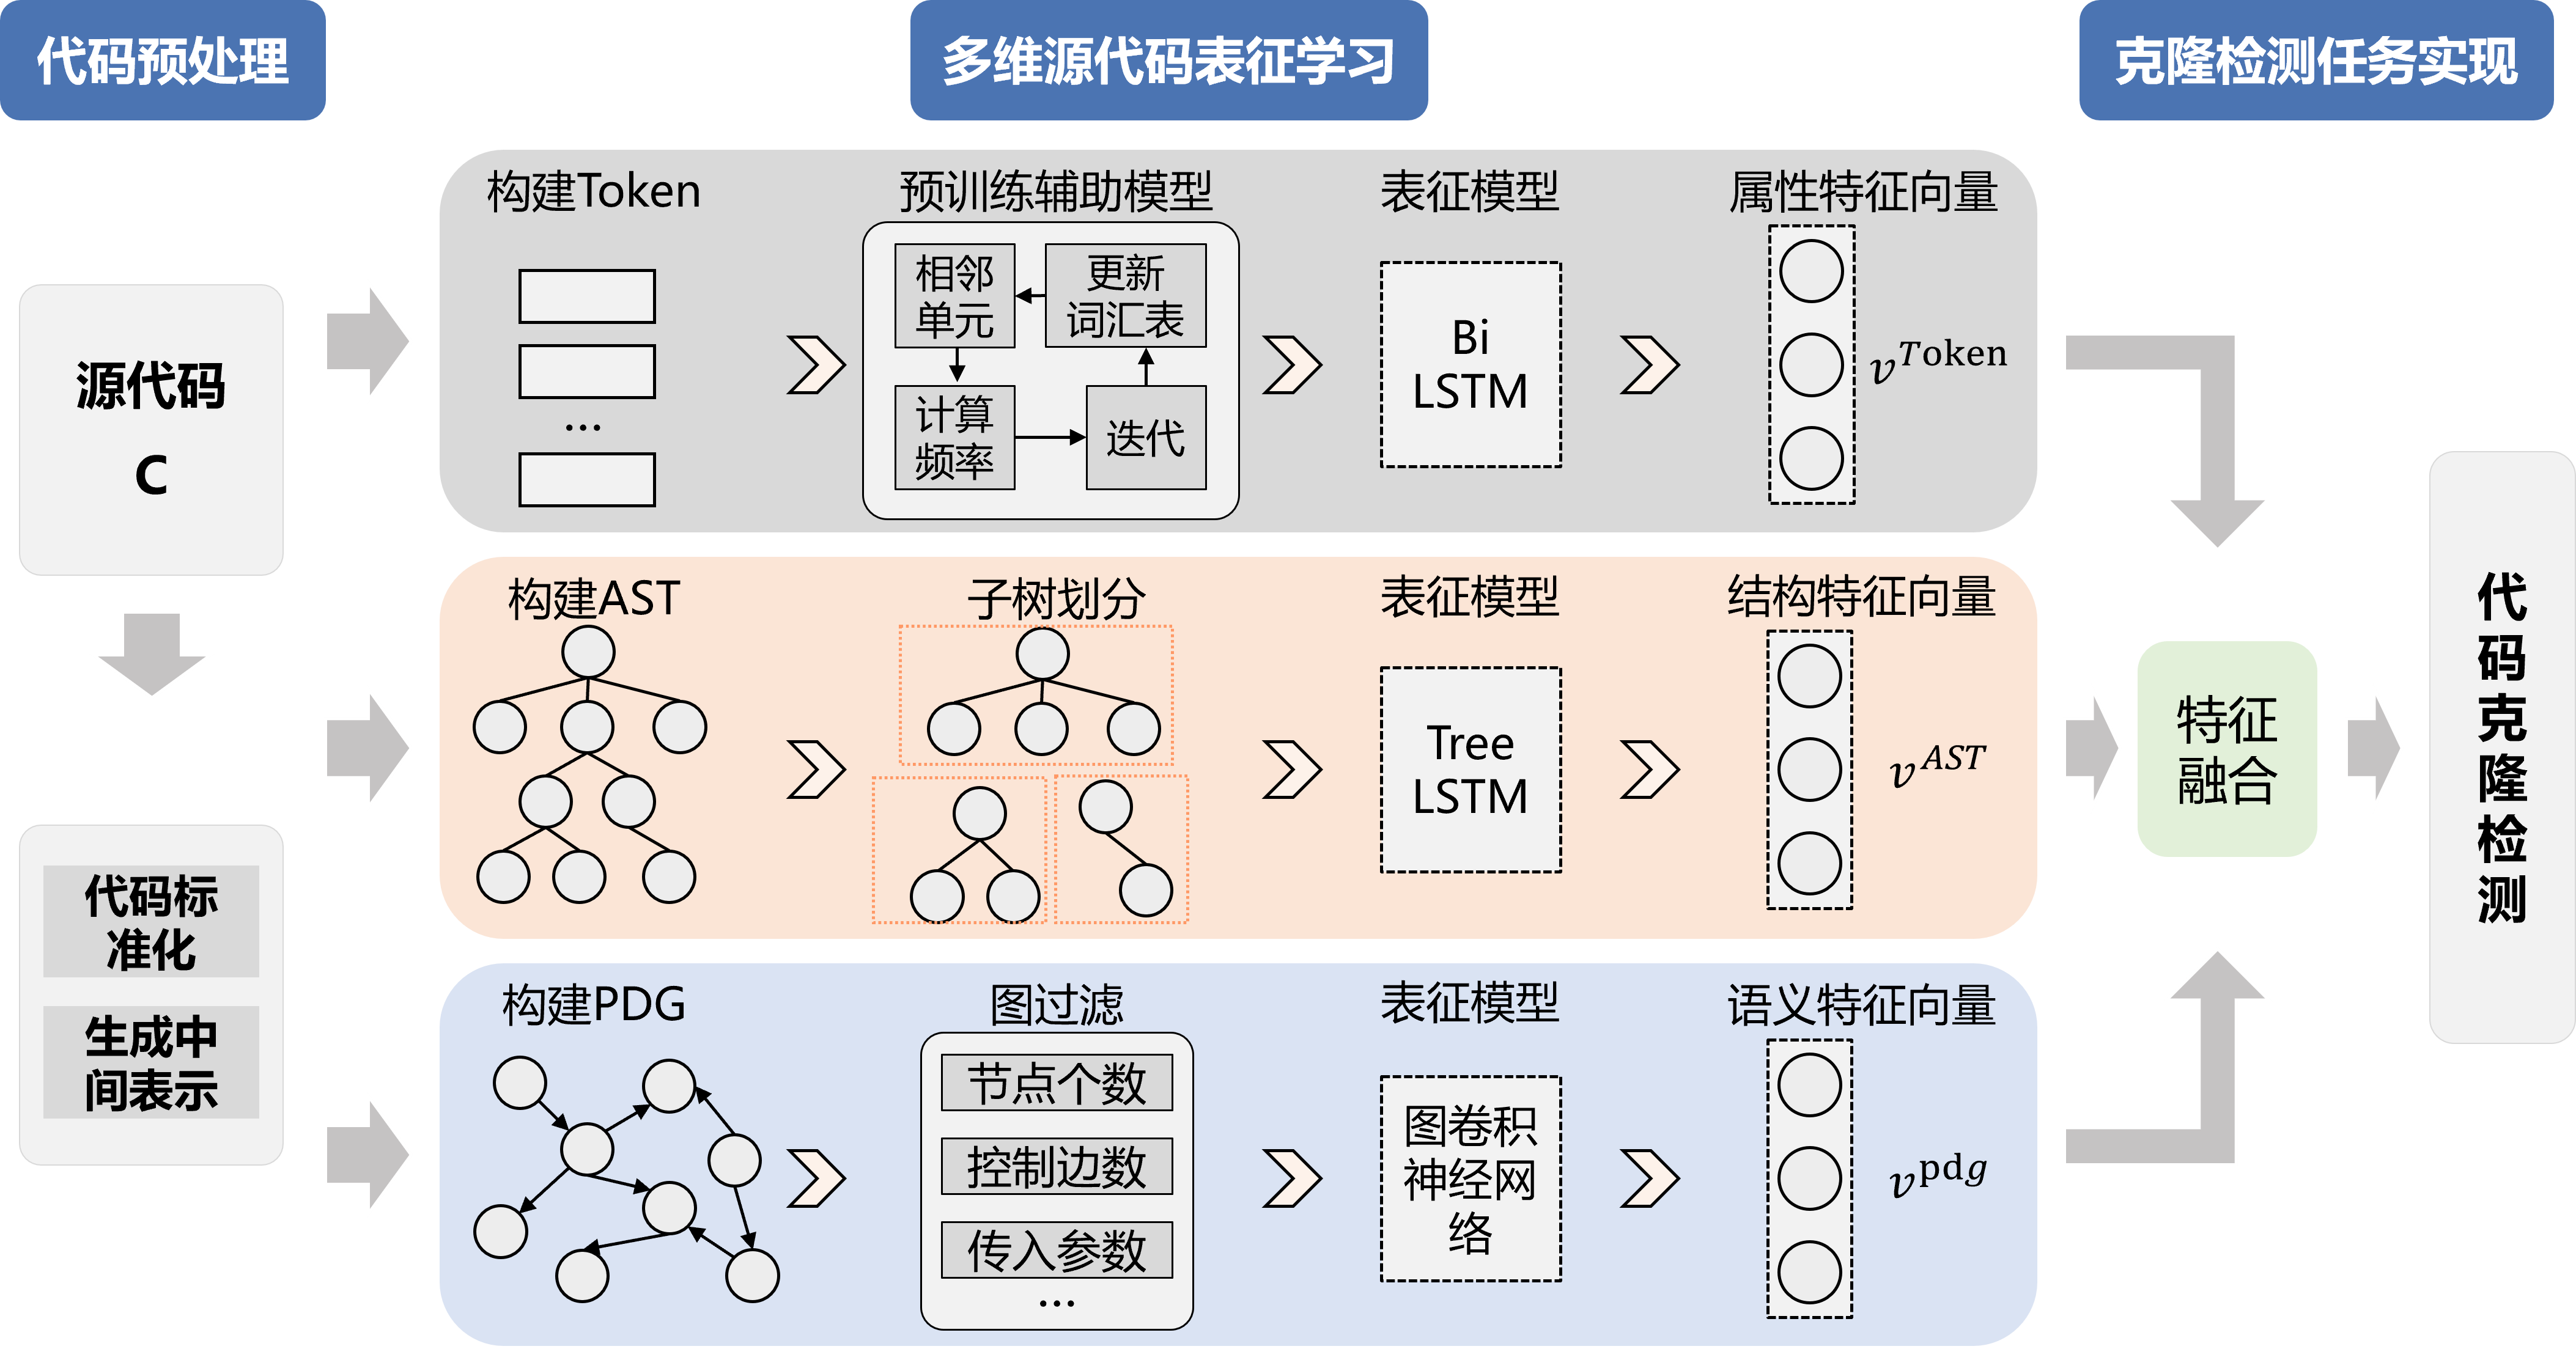
\includegraphics[width=0.75\textwidth]{figures/framework}
    \caption{RLCCD 总体框架}
    \label{fig:framework}
\end{figure}

\subsection{代码预处理}
\label{subsec:Preprocess}
代码预处理的目标是生成源代码片段对应的词法单元Token序列、抽象语法树AST和程序依赖图PDG,主要包含2个流程:代码标准化、生成中间表示。

(1)代码标准化

代码标准化的任务是去除与源代码无关的信息。首先是删除源代码片段中的注释、空行以及特殊符号,包括单行注释、多行注释、引入标准库的宏符号“\#”、无关符号等。其次,由于代码本身是一段包含丰富信息的文本,开发者通常会通过个人命名习惯对常量等标识符进行命名,这些私人信息并没有大多实际意义,反而会降低后续代码处理的精确率。因此,本文定义了一定的转换规则,将代码中的某些标识符转换为对应的标记,在最大限度地保留原有重要信息的同时,减少缺失关键语义联系。

(2)生成中间表示

基于标准化后的代码片段生成对应的中间表示:Token序列、抽象语法树AST和程序依赖图PDG。其中,词法单元Token序列可以通过词法分析器得到,词法分析器能够按照预定的语法规则将代码中的字符串分割为一个个词汇单元,这些词汇单元包含代码标准化处理后的标识符;抽象语法树AST以树状的形式抽象描述了程序语句的语法结构信息,生成抽象语法树时需要对源代码文本进行词法分析,然后依据语法规则分析整合Token,得到树型结构;程序依赖图PDG能够表示源代码的控制依赖,数据依赖赖等关系,是一种带有标记的有向多重图。生成程序依赖图时,需要对程序进行语法分析,然后分析程序中变量的关联关系,根据这种关联关系描绘程序的数据依赖和控制依赖关系,形成图的描述。

\subsection{多维源代码表征学习}
\label{subsec:Representation}
RLCCD框架的核心步骤是源代码表征学习,其目标是学习能够表示代码片段的连续向量,表现程序理解的认知层次,获取程序的语法、语义信息,创建程序更高抽象层次上的表示,它决定着对源代码信息抽取程度的上限,决定着检测方法的预处理方式、模型设计、部署方式、运行效率,并影响后续代码克隆检测任务所能检测的精度。本文提出的多维源代码表征学习方法包括Token序列、抽象语法树AST、程序依赖图PDG三种不同维度。下面详细介绍研究方案并分析其优化改进。

(1)词法单元Token

传统的基于Token的表征学习方法通常将代码表示为词汇单元,为了后续生成表征向量通常会将词汇单元规范化,丢失部分语法信息,出现在词汇表中不存在Token的难题。针对这样的问题,本文提出了一种预训练辅助模型的改进方法提取属性特征。具体来说,通过选取预训练辅助模型从代码语料库中学习基本单元的语法语义信息,以及这些单元之间的联系,最终给出一份单词-向量形式的词汇表,从而减少出现集外词问题的概率。

(2)抽象语法树AST

抽象语法树中包含了代码片段的结构信息,然而,传统的基于树的代码表征学习方法通常将抽象语法树转换为完整二叉树,可能破坏源代码原有的语法结构,增加AST高度,丢失长期上下文信息,削弱了神经网络模型捕捉更真实和复杂语义的能力,导致梯度消失的难题。针对这样的问题,本文提出子树划分的改进方法提取结构特征。具体来说,将每个大型的抽象语法树分解为小语句树序列,并通过捕获语句的词法和句法知识将每一个语句树都编码成一个向量。在得到一个语句向量序列后,将语句向量序列输入网络中生成代码片段的结构向量表示。这种细粒度的处理使得模型可以很好处理很深的抽象语法树,解决梯度消失问题。

(3)程序依赖图PDG

程序依赖图中包含代码片段的控制依赖,数据依赖赖等语义关系,然而,传统的基于图的代码表征学习方法通常采用图匹配算法将图中的控制流和数据流编码为一个紧凑的语义特征矩阵,矩阵中每个元素都是高维系数特征向量,面临消耗的时间、空间开销巨大的难题。针对这样的问题,本文提出了图过滤机制的改进方法提取语义特征。具体来说,根据PDG的节点个数、控制边数、执行边数、数据边数、声明节点数、函数调用数、传入参数、传出参数等代表特征进行过滤,减少模型的输入规模。

(4)特征融合方法

特征融合的目标是将提取到的属性特性、结构特征、语义特征合并,得到一个更能代表代码信息的多维特征,更具有判别能力。具体来说,通过三个不同维度得到属性特性、结构特征、语义特征,然后将三个特征映射到相同的特征空间内,最简单的例子是对多个代码特征进行串联,除此之外,还可以使用神经网络、概率图模型等融合方法,将向量融合作为一个混合多维表征,包括非结构化(顺序Token形式的代码)和结构化(抽象语法树和程序依赖图形式的代码)信息。该多维特征能够在低维空间中高效计算实体和关系的语义联系,挖掘代码节点间更全面、层次更深的关系信息,从而提高后续下游的代码克隆检测任务的准确率。

\subsection{克隆检测任务实现}
\label{subsec:Clone detection}
克隆检测任务实现的核心任务是判断两个代码片段是否是真克隆对。经过\ref{subsec:Preprocess}节代码预处理和\ref{subsec:Representation}节多维源代码表征学习两个步骤,可以得到对应的混合特征向量表示作为输入,然后计算这两个向量之间的相似性判断是否存在代码克隆。目前,常见的计算向量相似性的方法包括计算距离度量、相似性度量两种,向量的距离越近相似度越大。一些研究倾向于把程序表征为向量形式,使用余弦相似度、Jaccard相似度、欧几里得距离、汉明距离、曼哈顿距离等评估指标计算向量之间的相似度,当相似度大于某个固定阈值时则认为存在代码克隆。具体的,本文通过输入混合特征训练分类模型,以最小化模型损失为目标,完成代码克隆检测任务。

\section{RLCCD定义描述}
\label{sec:RLCCD flow}

为了更形象地描述代码克隆检测问题,本节首先给出示例源代码片段\ref{fig:code},其中,图\ref{fig:code1}、图\ref{fig:code2}、图\ref{fig:code3}是三个简单的代码片段,函数的主要功能为:计算$Data$数组的元素之和,其中图\ref{fig:code1}的第10-13行采用for循环,图\ref{fig:code2}的第9-13行采用while循环,这两个代码片段属于真克隆对;图\ref{fig:code2}的第9-14行采用for循环,但在内部需要判断result的现有状态,因此图\ref{fig:code1}和图\ref{fig:code3}的代码片段属于假克隆对。
\begin{figure}[H] 
  \centering  %居中
  \subfigure[C语言代码片段1]{   %第一张子图
      \centering    %子图居中
      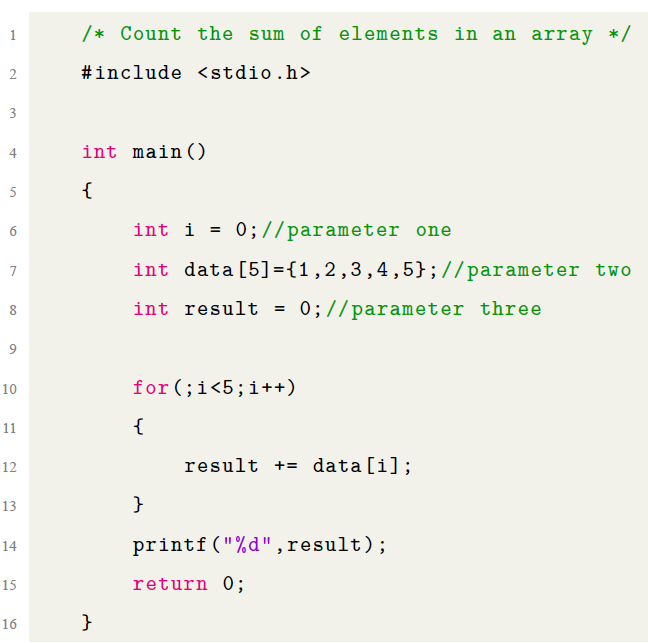
\includegraphics[width=0.3\textwidth]{figures/code1}
      \label{fig:code1} %引用标签
  }
  \subfigure[C语言代码片段2]{ %第二张子图
      \centering    %子图居中
      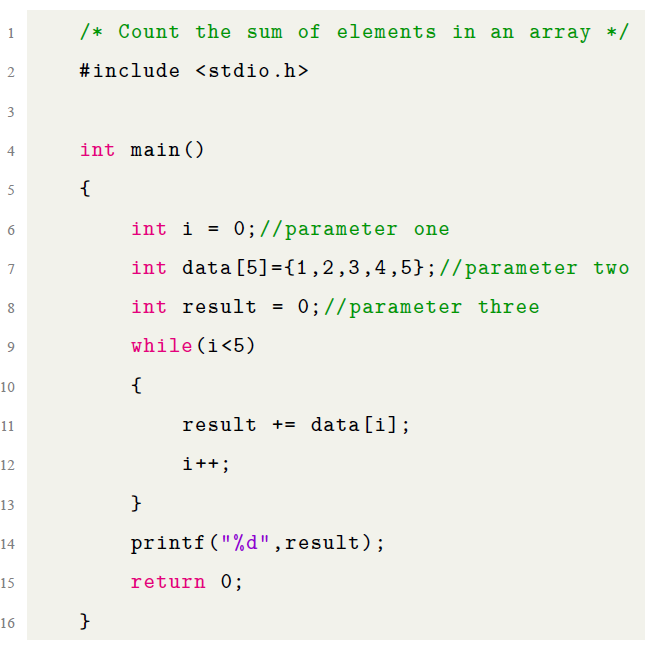
\includegraphics[width=0.3\textwidth]{figures/code2}
      \label{fig:code2} %引用标签
  }
  \subfigure[C语言代码片段3]{ %第三张子图
      \centering    %子图居中
      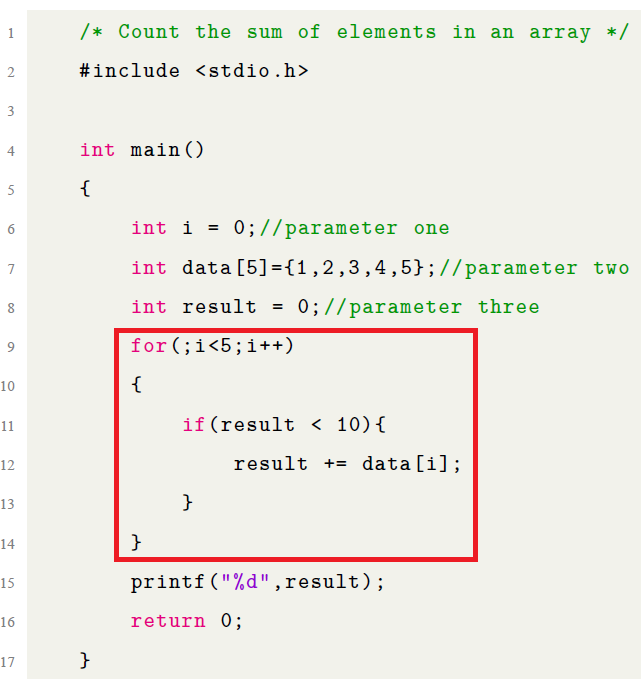
\includegraphics[width=0.3\textwidth]{figures/code3}
      \label{fig:code3} %引用标签
  }
  \caption{C语言代码片段示例}    %大图名称
  \label{fig:code}    %图片引用标记
\end{figure}
% \lstset{language=C}
% \begin{lstlisting}
%     /* Count the sum of elements in an array */
%     #include <stdio.h>
    
%     int main()
%     {
%         int i = 0;//parameter one
%         int data[5]={1,2,3,4,5};//parameter two
%         int result = 0;//parameter three
        
%         for(;i<5;i++)
%         {
%             result += data[i];
%         }
%         printf("%d",result); 
%         return 0;
%     }
% \end{lstlisting}

% \lstset{language=C}
% \begin{lstlisting}
%     /* Count the sum of elements in an array */
%     #include <stdio.h>
    
%     int main()
%     {
%         int i = 0;//parameter one
%         int data[5]={1,2,3,4,5};//parameter two
%         int result = 0;//parameter three
%         while(i<5)
%         {
%             result += data[i];
%             i++;
%         }
%         printf("%d",result); 
%         return 0;
%     }
    
% \end{lstlisting}

% \lstset{language=C}
% \begin{lstlisting}
%     /* Count the sum of elements in an array */
%     #include <stdio.h>
    
%     int main()
%     {
%         int i = 0;//parameter one
%         int data[5]={1,2,3,4,5};//parameter two
%         int result = 0;//parameter three
%         for(;i<5;i++)
%         {
%             if(result < 10){
%                 result += data[i];
%             }
%         }
%         printf("%d",result); 
%         return 0;
%     }
% \end{lstlisting}

给定两个代码片段$C_{a},C_{b}$,使用一个三元组$(C_{a},C_{b},y_{ab})$的形式来表示一对代码片段,其中$y_{ab}$表示标签。如果$(C_{a},C_{b})$是一个克隆对,那么$y_{ab}$为1,否则$y_{ab}$为0。从$n$个代码片段中构建一个带有标签的训练集$\left\{(C_{a},C_{b},y_{ab})|a,b \in n,a<b\right\}$,本文的目的是训练一个深度学习模型来学习一个可以把代码$C$映射成一个特征向量$V$的函数$f$。对于任意代码片段,计算出他们的相似度分数$S_{ab} = f(C_{a},C_{b})$并进行分类,使其分类结果尽可能接近已知的标签$y_{ab}$。在预测阶段,为了推断出两个代码片段是否是克隆对,在真假克隆对之间设置了一个阈值$k$,如果预测的相似度分数大于$k$值,那么认为两个代码片段是真克隆对,否则,认为它们是假克隆对。其中,训练一个深度学习模型将代码$C$映射成一个特征向量$V$的过程,可以视为代码表征学习的数值化过程,也是本文研究的重点。

面向代码克隆检测的多维源代码表征学习方法RLCCD架构如图\ref{fig:flow}所示,采用Siamese架构。RLCCD方法的输入是两个代码片段$C_{a},C_{b}$,输出是一个0或1的标签,1表示这两个代码片段是真克隆对,0表示是假克隆对。Siamese架构采用两个不同的输入,通过两个具有共享权值的相似子网络,输出一个编码来计算两个输入之间的相似度。整个方法的执行包括四个步骤,分别是:
\begin{figure}[H]
    \centering
    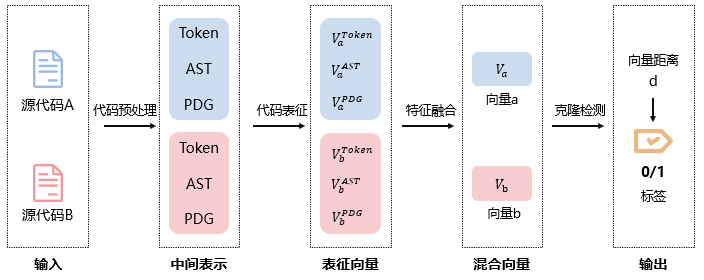
\includegraphics[width=0.95\textwidth]{figures/flow}
    \caption{面向代码克隆检测的多维源代码表征学习方法RLCCD架构图}
    \label{fig:flow}
\end{figure}

\textbf{代码预处理}:RLCCD接受两个代码片段$C_{a},C_{b}$作为输入,通过代码预处理阶段,得到对应的中间表示:词法单元Token序列、抽象语法树AST、程序依赖图PDG。

\textbf{代码表征}:代码表征是本文的核心步骤,输入是代码片段$C_{a},C_{b}$对应的中间表示,输出是对应的表征向量,分别记为代码片段$C_{a}$的属性特征$V_{a}^{Token}$、结构特征$V_{a}^{AST}$、语义特征$V_{a}^{PDG}$,代码片段$C_{b}$的属性特征$V_{b}^{Token}$、结构特征$V_{b}^{AST}$、语义特征$V_{b}^{PDG}$。

\textbf{特征融合}:特征融合阶段的输入是代码片段$C_{a},C_{b}$的特征向量,输出是对应的混合向量$V_{a},V_{b}$。本文将提取到的属性特性、结构特征、语义特征合并,得到一个更能代表代码信息的多维特征。我们用公式\ref{e4}表示特征融合。

\begin{equation}\label{e4}
    \setlength{\abovedisplayskip}{1pt}
    \mathrm{V}=W_{dt}\left[v^{\text{Token}} \bullet v^{\text{AST}} \bullet v^{\text{PDG}}\right]+b_{dt}
\end{equation}

其中$\bullet$表示特征融合方法,$V$表示最终的多维混合代码表示。$W_{dt}$在生成的多维混合表示中平衡属性特征$V^{Token}$、结构特征$V^{AST}$、语义特征$V^{PDG}$的组成,而$b_{dt}$在训练模型时使模型偏向最终收敛。

\textbf{克隆检测}:经过三个步骤,可以得到代码片段对应的向量表示$V_{a},V_{b}$。由于代码克隆检测问题是一个二分类问题,即给定两个代码片段,需要输出0或1,0表示它们之间不相似,1表示相似。因此通过公式\ref{e1}计算代码片段$C_{a}$对应的多维表征$V_{a}$与代码片段$C_{b}$对应的多维表征$V_{b}$之间的距离$d$,并将向量距离$d$映射到0$\sim$1之间,将输出值作为两个代码片段的相似度$S_{ab}$。
\begin{equation}\label{e1}
    \begin{split}
    d &= \left|V_{a}-V_{b}\right| \\
    \mathrm{S_{ab}} &=\operatorname{sigmoid}\left(d\right) \in[0,1]
    \end{split}
\end{equation}

并将损失函数定义为二元交叉熵,如公式\ref{e2}所示,训练模型的目标是最小化损失。
\begin{equation}\label{e2}
    J(\Theta, S_{ab}, y_{ab})=\sum(-(y_{ab} \cdot \log (S_{ab})+(1-y_{ab}) \cdot \log (1-S_{ab})))
\end{equation}

其中,$y_{ab}$表示两个代码片段的真实标签。

当所有参数都设置为最优化后,模型被存储起来。在预测阶段,通过公式\ref{e3}得到预测值。
\begin{equation}\label{e3}
    \text { prediction }=\left\{\begin{array}{ll}
        1, & S_{ab}>k \\
        0, & S_{ab} \leq k
        \end{array},\right.
\end{equation}

\section{本章小结}
\label{sec:Summary2}
本章首先给出了代码克隆检测问题的定义,然后分析了源代码表征学习在代码克隆检测过程中所面临的关键技术挑战,主要表现为Token集外词问题、树梯度消失问题、图规模开销、单个表征维度对代码信息利用率低问题。针对四个问题,本文提出了面向代码克隆检测的多维源代码表征学习方法RLCCD,在介绍了其整体框架后,对其中的关键技术点进行了简要的论述,最后详细描述了RLCCD的处理流程。
